\section{Künstliche Intelligenz}
\label{chap:KI}

Das Thema \ac{KI} hat in letzter Zeit durch den Chatbot ChatGPT der Firma OpenAI eine große mediale Aufmerksamkeit erhalten. 
ChatGPT wurde im November 2022 veröffentlicht und ist ein Sprachmodell, das natürliche Sprache verstehen und abhängig von der 
Benutzereingabe in Dialogform Antworten liefern soll. Es ist dabei in der Lage, sich an vorherige Eingaben zu erinnern und kann 
deshalb Anfragen in einen Kontext einordnen. Dadurch kann es auch vorherige Antworten korrigieren und auf Wünsche und Bedürfnisse 
des Benutzers eingehen \cite[]{CHATGPT}. 

Die Frage nach \ac{KI} und nach dem ob und wie Maschinen denken können ist jedoch wesentlich älter als dieser Chatbot. 
Bereits Alan Turing stellte sich diese Frage in den 1950er Jahren. Er schlug vor, die Frage, ob Maschinen denken können,
mit einer anderen Frage zu ersetzen. Dafür formulierte er das Problem mithilfe eines Spiels, dem \glqq Imitation Game\grqq{}, 
das heute eher als Turing-Test bekannt ist, um. Dieses Spiel wird mit drei Personen gespielt, einem Fragesteller, einem Mann und 
einer Frau. Ziel des Spiels ist es, dass der Fragesteller mithilfe von Fragen herausfinden muss, welche Person der Mann und welche Person 
die Frau ist. Der Mann soll dabei versuchen, dass der Fragesteller ihn fälschlicherweise als die Frau identifiziert, während die Frau versuchen soll, 
dass der Fragesteller sie korrekt als Frau identifiziert. Dafür befindet sich der Fragesteller in einem anderen Raum und die Fragen werden entweder 
über eine außenstehende weitere Person oder einem Fernschreiber übermittelt. Was würde nun passieren, wenn eine Maschine die Rolle des Manns übernehmen würde?
Würde der Fragesteller dann häufiger oder seltener gewinnen \cite[vgl. S.433f.]{TURING}? Alan Turing glaubte, dass eine Maschine dann als
intelligent bezeichnet werden könne, wenn eine Maschine in der Lage dazu ist, menschliches Verhalten zu imitieren.

\begin{wrapfigure}[7]{r}{\textwidth/2}
    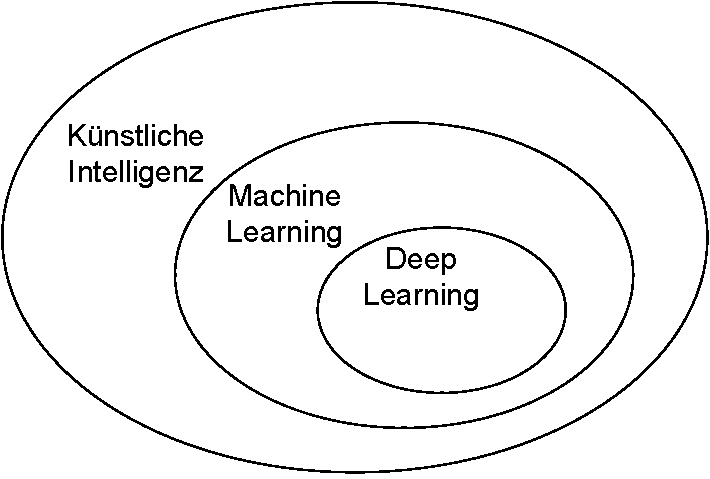
\includegraphics[width=\textwidth/2]{abbildungen/KI_ML_DL.pdf}
    \caption{Beziehung zwischen \ac{KI}, \ac{ML} und \ac{DL} \cite[vgl. S.22]{DL_PY}}
    \label{fig:KI_ML_DL}

\end{wrapfigure} 

François Chollet, der Entwickler der Deep-Learning-Bibliothek Keras, welche im Kapitel XXX TODO näher beschrieben wird, definiert
das Fachgebiet \ac{KI} als \glqq [den] Versuch, normalerweise von Menschen erledigte geistige Aufgaben automatisiert zu lösen\grqq{} \cite[S.22]{DL_PY}.
Nach dieser Definition schließt \ac{KI} weitere Themen wie das \ac{ML} sowie das \ac{DL} ein. Wichtig zu beachten ist dabei,
dass diese Gebiete sich voneinander unterschieden. Ihre Beziehung zueinander wird in Abbildung \ref*{fig:KI_ML_DL} verdeutlicht.\\

Dieses Kapitel wird näher erläutern, worum es sich bei den Themen \ac{ML} und \ac{DL} handelt und wie ein \ac{KI}-Modell als neuronales Netz erstellt wird.

\subsection{Maschinelles Lernen}

Das Maschinelle Lernen ist ein Teilgebiet der \ac{KI} und beschäftigt sich mit der Frage, ob ein Computer in der Lage dazu ist selbstständig eine bestimmte Aufgabe
zu erlernen. Ziel dabei ist es, dass eine Maschine aus einem vorgegebenem Datensatz und den dazugehörigen Antworten Regeln extrahieren soll, die den Datensatz erklären
können. Anders als bei der klassischen Programmierung soll eine Maschine hier nicht die Antworten aus den Daten und Regeln herausgeben, sondern selber nach einer
Struktur suchen, aus der die Maschine dann Regeln ableiten kann, die auch auf andere Aufgaben angewendet werden können \cite[vgl. S.23f.]{DL_PY}. Angenommen ein Datensatz bestünde aus
Bildern von Hunden und Menschen. Bei der klassischen Programmierung würde der Programmierer nun selber Regeln definieren und diese programmieren müssen. Beispiele für 
mögliche Regeln könnten hier sein:
\begin{quote}
    Wenn Wesen Fell hat, dann ist es ein Hund.\\
    Wenn Wesen auf zwei Beinen läuft, dann ist es ein Mensch.
\end{quote}
Beim \ac{ML} hingegen müsste der Programmierer diese Regeln nicht selber definieren. Hier werden neben dem Datensatz noch die entsprechenden Antworten benötigt. 
Jedes Bild bräuchte also ein Label, also eine Information darüber, ob es sich auf dem Bild um einen Hund oder einen Menschen handelt. Aufgabe der Maschine wäre es nun, 
mithilfe des Datensatzes und der Label, Regeln zu definieren, ob auf einem Bild ein Hund oder ein Mensch zu sehen ist. Das \ac{ML}-System wird also sozusagen trainiert. 
Dem trainiertem System können dann neue Bilder gezeigt werden und es wäre in der Lage anhand seiner definierten Regeln vorherzusagen, ob auf den neuen Bildern Hunde oder 
Menschen zu sehen sind. 

\begin{figure}[H]
    \centering
    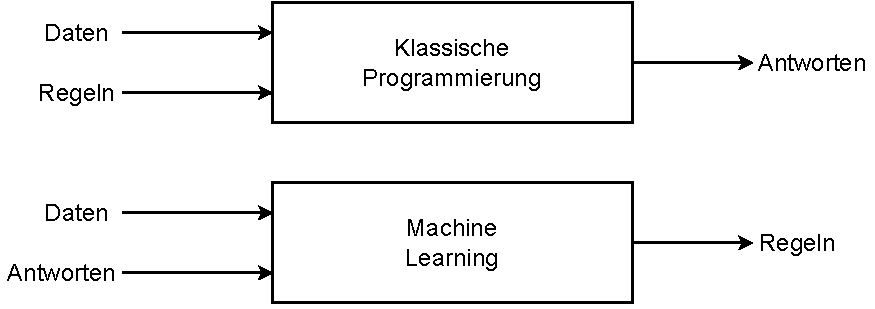
\includegraphics[scale=0.7]{abbildungen/Programmierparadigmen.pdf}
    \caption{Unterschiedliche Programmierparadigmen \cite[S.23]{DL_PY}}
    \label{fig:Programmierparadigma}
\end{figure}

Abbildung \ref*{fig:Programmierparadigma} verdeutlicht nochmal die Unterschiede zwischen der klassischen Programmierung und dem \ac{ML}. Beim \ac{ML} sind also drei Elemente
notwendig, diese werden anhand des oben genannten Beispiels verdeutlicht: 

\begin{description}[style=multiline,leftmargin=3cm,font=\bfseries]
    \item[Eingabedaten] Bilder von Menschen und Hunden \cite[S.24]{DL_PY}
    \item[Antworten] Label, ob auf dem Bild ein Mensch oder ein Hund abgebildet ist \cite[S.24]{DL_PY}
    \item[Metrik zur Bewertung des Algorithmus] Benötigt, um die Abweichung zwischen Ausgabe des Modells und eigentlicher Antwort zu bestimmen. Wird als Feedback-Signal genutzt,
    um Algorithmus anzupassen. Beispielsweise wie viel Prozent der Bilder richtig zugeordnet werden. \cite[S.24f.]{DL_PY}.  
\end{description}

Die Aufgabe eines \ac{ML}-Modells ist es passende Repräsentationen der Eingabedaten zu erlernen, das heißt, dass die Daten vom Modell sinnvoll umgewandelt werden müssen. 
Die systematische und automatische Suche nach der bestmöglichen Repräsentationen der Daten, mithilfe eines Feedback-Signals, für eine bestimmte vorgegebene Aufgabe kann als Möglichkeit verstanden werden, wie 
Maschinen lernen können. Mithilfe dieses Ansatzes und der in den letzten Jahren besser werdenden Hardware können große Datenmengen analysiert werden, was das Lösen von Aufgaben wie der Spracherkennung 
oder das autonome Fahren ermöglicht \cite[vgl. S.24ff.]{DL_PY}.\\

Die hier beschriebene Variante des Machine Learnings wird auch Supervised Learning, also überwachtes Lernen, genannt. \glqq Supervised\grqq{} bezieht sich hierbei darauf, dass
dem Modell die Antworten vorgegeben werden und es anhand der Antworten versucht Regeln zu finden. Neben dieser Variante existiert auch noch das sogenannte
Unsupervised Learning. Bei dieser Variante des Machine Learnings werden dem Modell keine Antworten gegeben. Stattdessen versucht das Modell die Daten anhand ihrer
Beziehung zueinander zu analysieren und die Daten in Kategorien zu klassifizieren. Algorithmen zum Clustern von Datensätze sind typische Beispiele für das Unsupervised Learning
\cite[vgl. S.47ff.]{AI_Huawei}. In dieser Arbeit finden Unsupervised Learning Algorithmen oder Modelle keine Anwendung, deshalb ist mit \ac{ML} hier immer Supervised Learning gemeint.

\subsection{Deep Learning}
